%!TEX root = ../dissertation.tex

\section{Epipolar Geometry}
\label{cha2:epipolar}

Epipolar geometry provides an alternative yet powerful tool to obtain image transformations using various different approaches. It describes the relation between two images, before and after a transformation, through a 3x3 singular, non-invertible, matrix called the \textbf{essential matrix}, \textbf{$E$}, if the camera matrix is known, or the \textbf{fundamental matrix}, \textbf{$F$}, otherwise. These matrices are singular because they express an under-constrained relationship between a point in one image and its possible location in the other image, which is not unique due to depth ambiguity. The essential matrix is the product of a rotation matrix and a \gls{skews}, whose determinant is zero, as it will be shown below. If a point in the real world, $M$, is projected as a point $\mathbf{{m}_1}$ in the first image, and point $\mathbf{{m}_2}$ in the second, then those points satisfy the epipolar relation
\begin{equation}
\label{sec2:eq:epipolar}
\mathbf{\tilde{m}_2}^T F \mathbf{\tilde{m}_1} = 0,
\end{equation}
\begin{figure}[h]
	\centering
	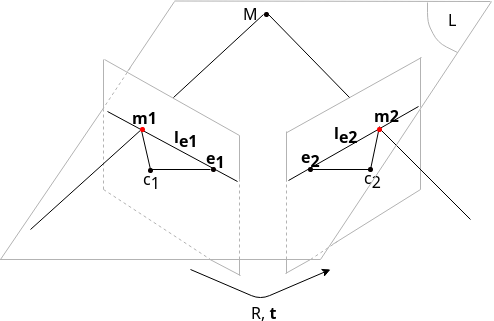
\includegraphics[width=11cm]{images/epipolargeo.png}
	\caption[Epipolar geometry]{Epipolar geometry. The two small vertical planes correspond to the image planes after the rotation and translation of the camera, $R$ and $\bf t$, respectively. $c_1$ and $c_2$ are the centers of projection before and after the transformation. $M$ is the fixed point gazed at in the real world. $\bf m_1$ and $\bf m_2$ are the projections of point $M$ into the respective image planes, whose rays are lying on the plane $L$. $\bf l_{e1}$ and $\bf l_{e2}$ are the epipolar lines, that also lie on the plane and $\bf e_1$ and $\bf e_2$ are the epipoles.}
	\label{sec2:fig:epipolargeo}
\end{figure}
which can be easily deduced with projective geometry. In Figure \ref{sec2:fig:epipolargeo}, $c_1$ and $c_2$ are the centers of projection before and after the camera has been displaced by $(R, \mathbf{t})$. Given the point $\bf m_1$ on the first image, its correspondence, $\bf m_2$, in the second image is constrained to a line, the epipolar line, $\bf l_{e2}$. The latter is defined as the intersection of the plane $L$ and the second image plane. Furthermore, plane $L$ is delineated by the two centers of projection and $\bf m_1$. The epipoles, $\bf e_1$ and $\bf e_2$, are born from the intersection of the line $c_1 - c_2$ with the epipolar lines, $\bf l_{e1}$ and $\bf l_{e2}$. 

\subsection{Projective geometry concepts}

To understand the upcoming deductions, let's introduce the following concepts.
\subsubsection{Representation of lines in \gls{homo}}
A line in a plane is represented by $a x + b y + c = 0$, which can also be defined by a vector $( a , b , c ) ^T$. For any non-zero constant, $k$, the vectors  $( a , b , c ) ^T$ and $k(a , b , c ) ^T$ represent the same line and are equivalent. An equivalence class of vectors is known as an homogenous vector. 
\subsubsection{Point lying on a line}
A point $\mathbf { p } = ( p_1 , p_2 ) ^ T$ lies on a line $\mathbf {\tilde{l}} = ( a , b , c ) ^ { T }$, if and only if $a p_1 + b p_2 + c = 0$, which can be written as $( p_1 , p_2 , 1 ) ( a , b , c ) ^T = \mathbf { \tilde{p} } ^T \mathbf {\tilde{l}} = \mathbf {\tilde{l}} ^T \mathbf { \tilde{p} } = 0$.
\subsubsection{Line joining points}
A line passing through any two points $\mathbf{\tilde{p}}$ and $\mathbf{\tilde{q}}$ can be defined by the cross-product of those points as $\mathbf{\tilde{l}} = \mathbf{\tilde{p}} \times \mathbf{\tilde{q}}$.
\subsubsection{Cross product's \gls{skews} representation}
The previous cross product, $\mathbf{\tilde{l}} = \mathbf{\tilde{p}} \times \mathbf{\tilde{q}}$, can be written as $\mathbf{\tilde{l}} = [\mathbf{\tilde{p}}]_{\times} \mathbf{\tilde{q}}$, where $[\mathbf{p}]_{\times}$ is a skew symmetric matrix defined as
\begin{equation}
\left[ \begin{array} { c c c } { 0 } & { - p_ { 3 } } & { p_{ 2 } } \\ { p_{ 3 } } & { 0 } & { - p_{ 1 } } \\ { - p _ { 2 } } & { p_ { 1 } } & { 0 } \end{array} \right]
\end{equation}.

\subsection{Deducing the fundamental matrix algebraically}

The derivation of the fundamental matrix uses the following facts,
\begin{enumerate}
	\item there is an \gls{homography} mapping via $L$ plane from the points of the first to the second image, characterized by $\mathbf{\tilde{m}_2} = H_M \mathbf{\tilde{m}_1}$;
	\item because $\mathbf{m_2}$ lies on $\mathbf{\tilde{l}_{e_2}}$, then $\mathbf{ \tilde{m}_2 } ^T \mathbf{\tilde{l}_{e_2}} = 0$;
	\item and since $\mathbf { e_2 }, \mathbf { m_2 } \in \mathbf{\tilde{l}_{e_2}}$, then $\mathbf{\tilde{l}_{e_2}} = [\mathbf{\tilde{e}_2}]_{\times} \mathbf{\tilde{m}_2}$.
\end{enumerate}
From 1) and 3), 
\begin{equation}
\label{ggg}
\mathbf{\tilde{l}_{e_2}} = [\mathbf{\tilde{e}_2}]_{\times} H_M \mathbf{\tilde{m}_1} 
\end{equation}
can be deduced and using conclusion 2) and (\ref{ggg}),
\begin{equation}
\label{sec2:eq:fundm}
\mathbf{\tilde{m}_2}^T \mathbf{\tilde{l}_{e_2}} = 0 = \mathbf{\tilde{m}_2}^T [\mathbf{\tilde{e}_2}]_{\times} H_M \mathbf{\tilde{m}_1}  = \mathbf{\tilde{m}_2}^T F \mathbf{\tilde{m}_1},
\end{equation}
where $F$, the fundamental matrix, is an homogeneous matrix of rank-2 (since $[\mathbf{\tilde{e}_2}]_{\times}$ is rank-2 and $H_M$ is rank-3) with 7 degrees of freedom, and $det(F) = 0$.

\subsection{Deducing the fundamental matrix from camera motion}
Another way of obtaining this relation is through the camera motion.
If the point in the real world is expressed in the eye's perspective before rotating, $M_1$, under the camera model studied in section \ref{cha2:features}, (\ref{sec2:eq:eproj1}) and ((\ref{sec2:eq:eproj2}) are true and (\ref{sec2:eq:eproj3}) can be derived from them.
\begin{align}
\label{sec2:eq:eproj1}
\lambda_1 \mathbf{\tilde{m}_1} = K \tilde{M_1}, \\
\label{sec2:eq:eproj2}
\lambda_2 \mathbf{\tilde{m}_2} = K [ R \ \mathbf{t} ] \tilde{M_1}\\
\label{sec2:eq:eproj3}
\lambda_2 \mathbf{\tilde{m}_2} = K [ R \ \mathbf{t} ] K^{-1} \lambda_1 \mathbf{\tilde{m}_1}
\end{align}
For the sake of simplicity, the intrinsics matrix will be considered the identity, $K= I$, and the scale factors $\lambda_1$ and $\lambda_2$ will be dropped. Hence, by eliminating $\tilde{M_1}$, the previous equations become
\begin{equation}
\label{sec2:eq:elimp}
\mathbf{\tilde{m}_2} = R   \mathbf{\tilde{m}_1} + \mathbf{t},
\end{equation}
and because the cross product of two vectors is orthogonal to them both,  
\begin{align}
	\label{sec2:eq:fundm1}
	\mathbf{\tilde{m}_2}^T \cdot ( \mathbf{\tilde{m}_2} \times \mathbf{t}) = 0 \\
	\label{sec2:eq:fundm2}
	\text{and } ( \mathbf{\tilde{m}_2}^T\cdot((R  \mathbf{\tilde{m}_1} + \mathbf{t}) \times \mathbf{t}) = 0.
\end{align}
Therefore, the fundamental matrix, $F$, can be determined by 
\begin{equation}
\label{sec2:eq:fundm3}
\begin{aligned}
\mathbf{\tilde{m_2}}^T [\mathbf{t}]_\times R \mathbf{\tilde{m_1}} = 0 \\
\mathbf{\tilde{m_2}}^T F \mathbf{\tilde{m_1}} = 0.
\end{aligned}
\end{equation}
When the intrinsic parameters are not the identity matrix, then 
\begin{equation}
\begin{aligned}
\label{hhh}
\mathbf{\tilde{m_2}}^T K^{-T} E K^{-1} \mathbf{\tilde{m_1}} = 0 \\
\text{and finally }
F = K^{-T}  E K^{-1},
\end{aligned}
\end{equation}
where $E$ is the essential matrix.

\subsection{Estimating the fundamental matrix}
\label{einvonrev}
Having seen how the fundamental matrix is obtained from the known rotation and translation of a camera, the question now is how to determine $F$, and consequently the rotation, given two images with matching points. With the points referred to as $\mathbf{m_{1}} = [u_{1} \ v_{1}]^T$ and $\mathbf{m_{2}} = [u_{2}  \ v_{2}]^T$, the epipolar equation (\ref{sec2:eq:epipolar}) can then be written as
\begin{equation}
\begin{aligned}
\begin{bmatrix}
u_2 & v_2 & 1
\end{bmatrix}
\begin{bmatrix}
f_{11} & f_{12} & f_{13}  \\
f_{21} & f_{22} & f_{23}  \\
f_{31} & f_{32} & f_{33} 
\end{bmatrix}
\begin{bmatrix}
u_{1} \\ v_{1} \\ 1
\end{bmatrix}\\
=
\begin{bmatrix}
f_{11} u_1 u_2 + f_{12} v_1 u_2  + f_{13}u_2 + f_{21} u_1 v_2  + f_{22} v_1 v_2  + f_{23}v_2  + f_{31} u_1 + f_{32} v_1 + f_{33} 
\end{bmatrix}\\
=
\begin{bmatrix}
u_1u_2 \ v_1u_2 \ u_2 \ u_1v_2 \ v_1v_2 \  v_2 \ u_1 \ v_1 \ 1 
\end{bmatrix}
\begin{bmatrix}
f_{11} \ f_{12} \ f_{13} \ f_{21} \ f_{22} \ f_{23} \ f_{31} \ f_{32} \ f_{33}
\end{bmatrix}^T\\
= \mathbf{u} \cdot \mathbf{f}\\ = 0
\end{aligned}
\end{equation}
For $n$ pairs of points the expression becomes 
\begin{equation}
\label{sec2:eq:nsets}
U f = 0,
\end{equation}
where $U = \left[ \mathbf{u_ { 1 }} , \cdots , \mathbf{u_ { n }} \right] ^ { T }$. 
This linear homogeneous equation, and the rank-2 constraint over $F$, that restrains the matrix to 7 degrees of freedom (since $F$ is also defined up a scalar factor), will permit its unique identification. 
Hence, the estimation of $F$ may be done using only 7 point matches, or by using 8 or more if enough data points are available. In the latter case, the solution produced is in general unique, and there are several techniques to obtain it. In Zhang 1996's review on the issue \cite{detep}, the conclusion was that linear techniques are usually sensitive to noise and not very stable, because they ignore the constraints of $F$ and the minimization criterion is not physically meaningful. However, the results could be improved by using normalized data points instead of pixel coordinates. 

Nevertheless, non-linear optimization techniques seem to yield better results to the estimation problem of $F$. Three nonlinear algorithms are mentioned in the review paper \cite{detep} and in R. Hartley and A. Zisserman \cite{multiview}: (i) a minimization of the re-projection errors, (ii) a minimization of the symmetric epipolar error, (iii) and a minimization of the first order geometric error. The first one is the most time-consuming, thus not recommended. From the other two most promising approaches, the second seems to give the worst results and the last algorithm has been proposed to give the best results in the least amount of computational time. 

Algorithm (i), also called the Gold Standard, estimates $F$ by minimizing the distances between the points in the image and its re-projections. Having $M_1$ as a point in space, the corresponding points in the images before and after rotating are $\widetilde{\mathbf{m}}_{1}$ and $\widetilde{\mathbf{m}}_{2}$, respectively, obtained through  (\ref{sec2:eq:eproj1}) and ((\ref{sec2:eq:eproj2}).
The re-projections of $\widetilde{\mathbf{m}}_{1}$ and $\widetilde{\mathbf{m}}_{2}$ are then, 
\begin{align}
\label{cha2:epipolar:shitshit1}
	\lambda_2 \mathbf{\tilde{m}^r_2} = K [ R \ \mathbf{t} ] K^{-1} \lambda_1 \mathbf{\tilde{m}_1}\\
\label{cha2:epipolar:shitshit2}
	\lambda_1 \mathbf{\tilde{m}^r_1} =  K [ R^{T} \ -R^{T}\mathbf{t} ] K^{-1}  \lambda_2 \mathbf{\tilde{m}_2},
\end{align}
where $R$ and $\mathbf{t}$ are obtained from the factorization of $F$, that will be approached briefly on section \ref{cha2:epipolar:fact}, $K$ are the known intrinsic parameters of the camera and $\lambda_1$ and $\lambda_2$ are given by the projection of the points on a sphere mentioned on section \ref{cha2:opprandsphere}. The distance between $\widetilde{\mathbf{m}}_{1}$ and $\widetilde{\mathbf{m}}^r_{1}$ is defined by $|| \widetilde{\mathbf{m}}_{1} - \widetilde{\mathbf{m}}^r_{1} ||$, leading to the following cost function to minimize 
\begin{equation}
\label{cha2:sec3:eq:gold}
	\min_{\mathbf{F}} \sum_{i}
	||\widetilde{\mathbf{m}}_{1i} - \widetilde{\mathbf{m}}^r_{1i}||^2
	+
	||\widetilde{\mathbf{m}}_{2i} - \widetilde{\mathbf{m}}^r_{2i}||^2,
\end{equation}
where $i=1,...,n$.

Algorithm (ii) minimizes the epipolar error symmetrically, which is the distance from a point to its epipolar line. Having the epipolar line of the first image as $\widetilde{\mathbf{l}}_{e_1} =  F\widetilde{\mathbf{m}}_{2}$ and the second's as $\widetilde{\mathbf{l}}_{e_2} =  F\widetilde{\mathbf{m}}_{1}$, as shown on \ref{sec2:eq:fundm}, the quantity to minimize is given by
\begin{equation}
	\min _{\mathbf{F}} \sum_{i}\left(d^{2}\left(\mathbf{m}_{2i}, \mathbf{l}_{e_{2}}\right)+d^{2}\left(\mathbf{m}_{1i}, \mathbf{l}_{e_{1}}\right)\right),
\end{equation}
where $d\left(\mathbf{p}, \mathbf{l}\right)=\frac{a p_{1}+b _{2}+c}{\sqrt{a^{2}+b^{2}}}$, with $\widetilde{\mathbf{l}} = (a, b, c)^{T}$
and $\mathbf{p}=\left(p_{1}, p_{2}\right)^{T}$, is the distance of a point to a line.

Minimizing $ \sum_i (\mathbf{\widetilde{m_i}}'^T F \mathbf{\widetilde{m_i}})^2$ doesn't yield a good result because the variance of each $i$ term is not the same and the least-squares technique produces an optimal solution if each term has the same variance. So one possibility is to determine the fundamental matrix the way it's given by algorithm (iii), 
\begin{equation}
\min_F \sum_i \frac{ (\mathbf{\widetilde{\mathbf{m}}_{2i}}^T F \widetilde{\mathbf{m}}_{1i})^2}{\sigma_i^2},
\end{equation}
where $\sigma_i^2$ is the variance given by 
\begin{equation}
\sigma_i^2 = \sigma [l_{{e1i}_x}^2 + l_{{e1i}_y}^2 + l_{{e2i}_x}^2 + l_{{e2i}_y}^2].
\end{equation}
This corresponds to minimizing the derivative of the epipolar relation, thus its also called \acrfull{grat}, or the Sampson error.
Because multiplying each term by a constant makes no difference, $\sigma$ can be dropped. 

\subsection{Factorization of the essential matrix}
\label{cha2:epipolar:fact}
Once the fundamental matrix is obtained through one of those methods, assuming the intrinsic parameters are known, which is the case for this work, the essential matrix may be obtained by $E = K^{T}  F K$ as seen on (\ref{hhh}).
From here, it's possible to retrieve the camera matrix, $P = [R \ | \ \mathbf{t}]$, since $E = [\mathbf{t}]_\times R$, so that the rotation, $R$, and thus the orientation of the camera becomes known.
To find the camera matrix, one can apply the \acrshort{svdd} to the essential matrix, which generates 4 possible solutions,
\begin{equation}
P = \left[UWV^T | + u_{ 3 } \right] \quad \text { or } \quad \left[ UWV^T | - u_ { 3 } \right] \quad \text { or } \quad \left[ UW^T V^T | + u_ { 3 } \right] \quad \text { or } \quad \left[ UW^T V^T |- u _ { 3 } \right],
\end{equation}
that are represented by (a), (b), (c) and (d), respectively, on Figure \ref{sec2:fig:ep4} \footnote{The way this solutions are obtained is further detailed on appendix \ref{appendix:cha1:epipolar}.}. $U$ and $V$ are the outputs of \acrshort{svdd} and 
\begin{equation}
	\mathrm { W } = \left[ \begin{array} { c c c } { 0 } & { - 1 } & { 0 } \\ { 1 } & { 0 } & { 0 } \\ { 0 } & { 0 } & { 1 } \end{array} \right] \quad.
\end{equation}
The real world point is only in front of both cameras in one of the four solutions, thus it is enough to use a single point to decide which of the different solutions produces the correct camera matrix. \cite{multiview}\\

To summarize, the steps for obtaining the camera matrix from epipolar geometry are:

\begin{enumerate}
	\item Determining the fundamental matrix, $F$, using one of the algorithms described on section \ref{einvonrev};
	\item Obtain the essential matrix, $E$, from the intrinsic parameters (which is possible in this case);
	\item Retrieve the four possible solutions for $P = [R \ | \ \mathbf{t}]$ by doing a \acrshort{svdd} decomposition on $E$;
	\item Choose the feasible solution.
\end{enumerate}

\begin{figure}[ht]
	\centering
	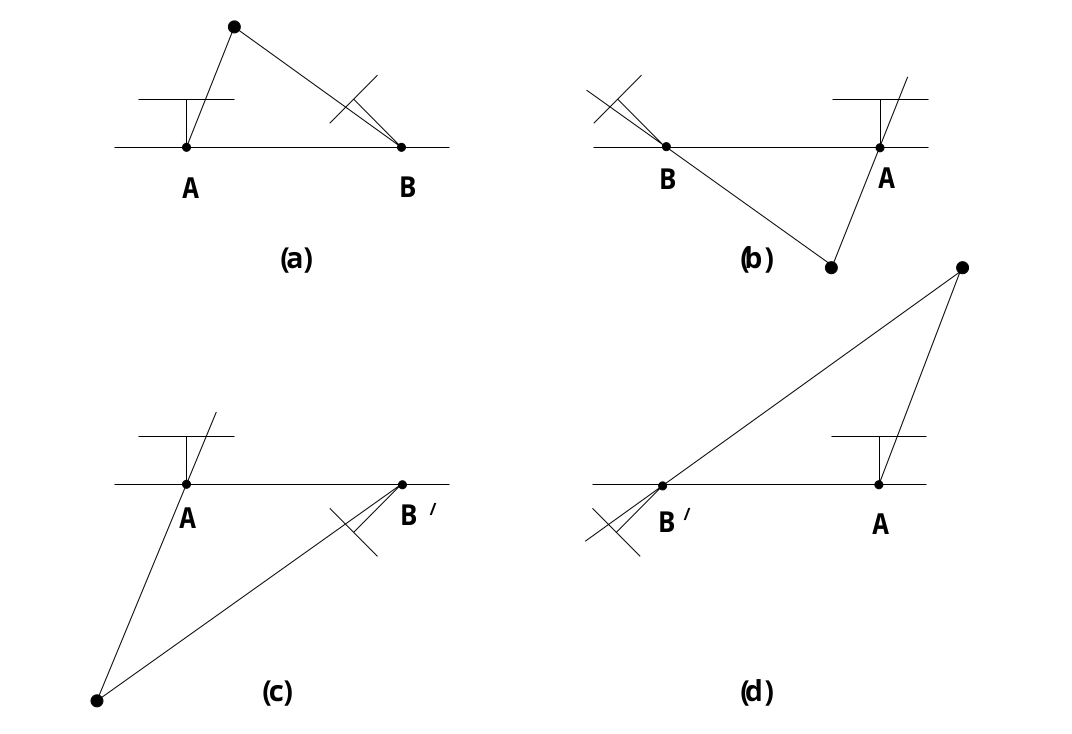
\includegraphics[width=10cm]{images/ep4sols.png}
	\caption[Four possible solutions retrieved from $E$]{Four possible solutions retrieved from the essential matrix $E$. The points A and B correspond to the centers of projection before and after rotating. Between the right side, (a) and (c), and the left side, (b) and (d), figures, there is a translation direction inversion. Between top, (a) and (b), and bottom, (c) and (d), figures, there is a rotation of 180 degrees around the baseline. \cite{multiview}}
	\label{sec2:fig:ep4}
\end{figure}

\subsection{Pure rotation}
\label{urerrrrr}
As a disadvantage of epipolar geometry, if the eye's movement is not constrained by a translation component, the epipolar relation will not work, since $[\mathbf{t}]_\times$ would be a $3x3$ matrix of zeros and, consequently, $E = [\mathbf{t}]_\times R$ would yield the same, making it impossible to retrieve the rotation.\\

When doing feature detection and matching, wrongly matched pairs of points between the two images, or points with large location errors, could severely affect the precision of the estimation of $F$. The reason for this is that all methods are least-square techniques that assume the noise which corrupts the data has zero mean. Hence, it is relevant to look into techniques of robust estimation.

